\begin{sol}
\begin{enumerate}[label=\textbf{(\alph*)}]
\item
$$\forall u\in\mathbb U, |v-u|\geq|v-P_U v|$$ 
The orthogonal projector acting on a vector $v=u+w, u\in\mathbb U, w\in\mathbb U^\perp$ will result in $P_Uv=u$.
$$\braket{v-u}{v-u}\geq\braket{v-P_Uv}{v-P_Uv}$$
$$\braket{v}{v}+\braket{u}{u}-\braket{u}{v}-\braket{v}{u}\geq\braket{v}{v}+\braket{P_Uv}{P_Uv}-\braket{P_Uv}{v}-\braket{v}{P_Uv}$$
$$\braket{u}{u}-2\mathrm{Re}\braket{u}{v}\geq\braket{P_Uv}{P_Uv}-2\mathrm{Re}\braket{P_Uv}{v}$$
Rewrite $v=P_uv+w, w\in\mathbb U^\perp$
$$\braket{u}{u}-2\mathrm{Re}\braket{u}{P_Uv+w}\geq\braket{P_Uv}{P_Uv}-2\mathrm{Re}\braket{P_Uv}{P_Uv+w}$$
$$\braket{u}{u}-2\mathrm{Re}\braket{u}{P_Uv}-2\mathrm{Re}\braket{u}{w}\geq\braket{P_Uv}{P_Uv}-2\mathrm{Re}\braket{P_Uv}{P_Uv}-2\mathrm{Re}\braket{P_Uv}{w}$$
The inner product of a vector with itself must be real, thus, $\mathrm{Re}\braket{v}{v}=\braket{v}{v}$.
$$\braket{u}{u}-2\mathrm{Re}\braket{u}{P_Uv}\geq-\braket{P_Uv}{P_Uv}$$
$$\braket{u}{u}-2\mathrm{Re}\braket{u}{P_Uv}+\braket{P_Uv}{P_Uv}\geq 0$$
$$|u-P_Uv|^2\geq 0$$ 
\item
Let $\ket{e_1}= \alpha\ket{1}$
$$\braket{e_1}{e_1}=1\implies \alpha^2\int_{-\pi}^\pi dx=1, 2\pi\alpha^2=1$$ $$\alpha=\frac{1}{\sqrt{2\pi}}$$ $$\ket{e_1}=\frac{1}{\sqrt{2\pi}}\ket 1$$
$$\ket{e_2}=\frac{\ket x-\braket{e_1}{x} \ket{e_1}}{|\ket x-\braket{e_1}{x} \ket{e_1}|}$$
$$\braket{e_1}{x}=\int_{-\pi}^\pi \frac{x}{\sqrt{2\pi}}=0
\,\,\,\,\,\, \braket{x}{x}=\int_{-\pi}^\pi x^2 dx=\frac{2\pi^3}{3}$$$$\ket{e_2}=\sqrt{\frac{3}{2\pi^3}}\ket x$$ 
The similar procedure can be applied to obtained $\ket{e_3}...\ket{e_6}$ to obtain
$$\ket{e_3}=\sqrt{\frac{5}{8\pi^5}}(3\ket{x^2}-\pi^2\ket 1)$$
$$\ket {e_4}=\frac{25}{2}\sqrt{\frac{7}{2\pi^7}}(5\ket{x^3}-3\pi^2\ket x)$$ $$\ket{e_5}=\frac{3}{8\sqrt{2\pi^9}}(35\ket{x^4}-30\pi^2\ket{x^2}+3\pi^4\ket 1)$$ 
$$\ket{e_6}=\frac{1}{8}\sqrt{\frac{11}{2\pi^{11}}}(63\ket{x^5}-70\pi^2\ket{x^3}+15\pi^4\ket{x})$$ 
\item
$$\ket{\sin x}\approx(\ketbra{e_1}{e_1}+\ketbra{e_2}{e_2}+...+\ketbra{e_6}{e_6})\ket{\sin x}$$ $$=\frac{21x}{8\pi^{10}}\Big(33x^4(\pi^4-105\pi^2+945)-30\pi^2x^2(\pi^4-125\pi^2+1155)+5\pi^4(\pi^4-153\pi^2+1485)\Big)$$
$$\approx 0.00564312x^5-0.155271x^3+0.987862x$$ $$\ket{\cos x}\approx(\ketbra{e_1}{e_1}+\ketbra{e_2}{e_2}+...+\ketbra{e_6}{e_6})\ket{\cos x}$$$$=\frac{105}{8\pi^8}\Big(315 x^4 - 30 \pi^2 x^2 (9 + x^2) + 3 \pi^4 (9 + 8 x^2)-2 \pi^6\Big)$$ $$\approx 0.0261598x^4-0.452288x^2+0.978326$$ 
\item 
Plot of $\sin x$: Green-second degree, Yellow-fourth degree, Red-fifth degree, Blue-actual\\
\begin{center}
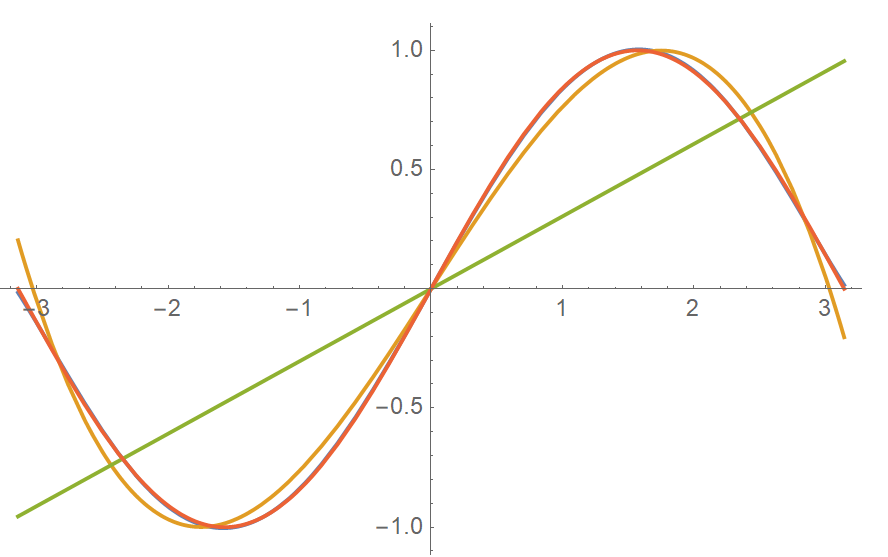
\includegraphics[scale=0.7]{P04/sinx.PNG}
\end{center}
Error (fifth degree): Blue-approximation in $\mathbb U$, yellow-taylor polynomial
\begin{center}
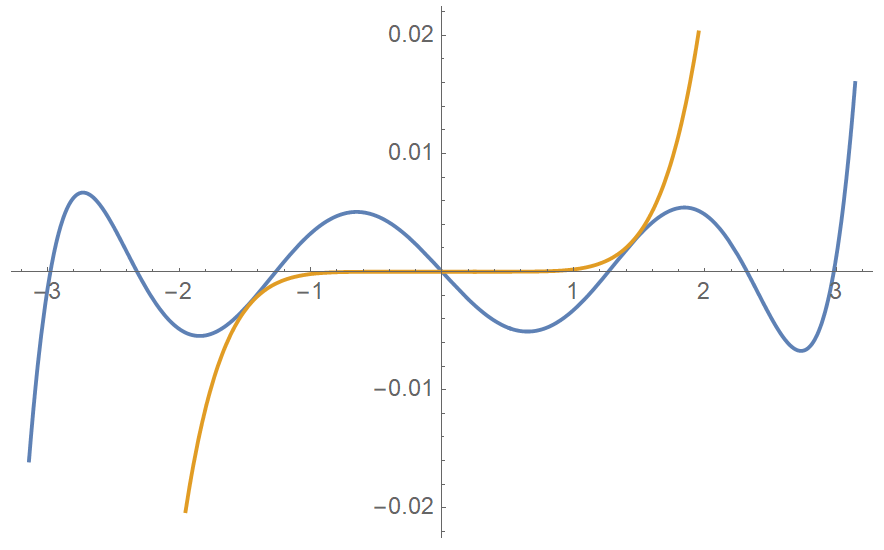
\includegraphics[scale=0.7]{P04/sin error.PNG}
\end{center}
Plot of $\cos x$: Yellow-third degree, Green-fifth degree, Blue-actual
\begin{center}
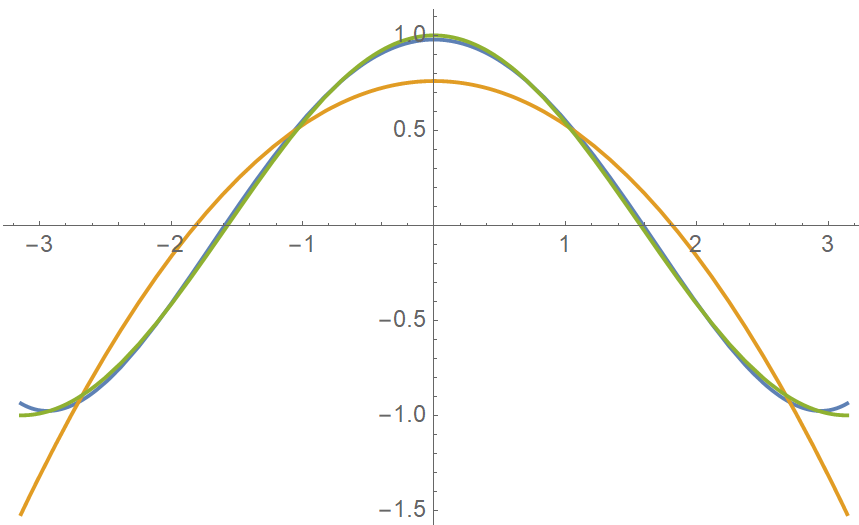
\includegraphics[scale=0.7]{P04/cosx.PNG}
\end{center}
\newpage
Error (fifth degree): Blue-approximation in $\mathbb U$, yellow-taylor polynomial
\begin{center}
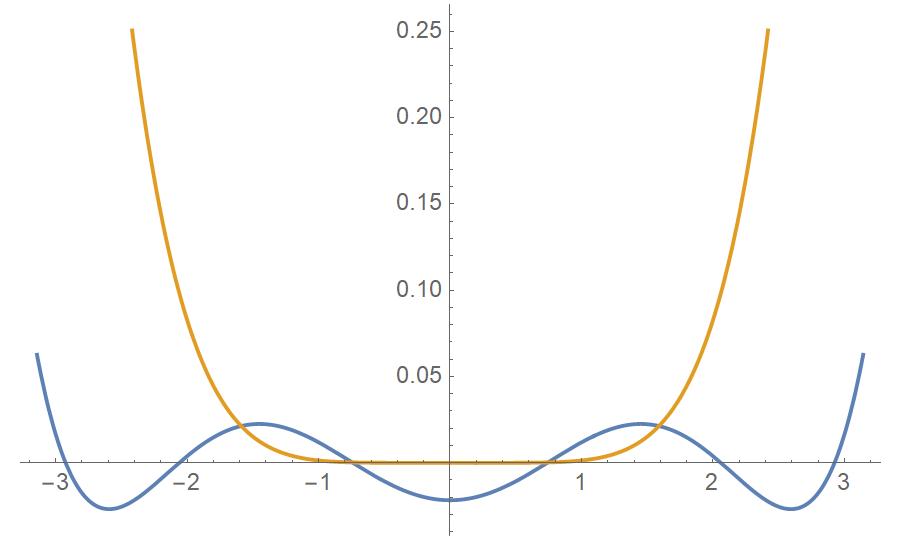
\includegraphics[scale=0.7]{P04/cos error.PNG}
\end{center}
In conclusion, the approximation in the space $\mathbb U$ is a better approximation if the entire interval $(-\pi,\pi)$ is considered whereas the taylor polynomial is a better approximation near zero. 

\end{enumerate}
\end{sol}